%Przykładowy plik ułatwiający złożenie projektu dyplomowego inżynierskiego.
%UWAGA: Generowany napis na stronie tytułowej o treści PROJEKT DYPLOMOWY INŻYNIERSKI został zaproponowany przeze mnie i nie jest, póki co, potwierdzony przez władze wydziału. Przed ostatecznym oddaniem tak złożonej pracy należy upewnić się jaka powinna być treść tego napisu. W momencie gdy uzyskam informację na temat treści tego napisu, dokonam niezbędnych zmian w źródłach.

\documentclass[en,printmode]{mgr}
%opcje klasy dokumentu mgr.cls zostały opisane w dołączonej instrukcji

%poniżej deklaracje użycia pakietów, usunąć to co jest niepotrzebne
%\usepackage{polski} %przydatne podczas składania dokumentów w j. polskim
\usepackage[utf8]{inputenc}
\usepackage[T1]{fontenc} %poprawne składanie polskich czcionek
%pakiety do grafiki
\usepackage{graphicx}
\usepackage{subcaption}
\usepackage{psfrag}

%pakiety dodające dużo dodatkowych poleceń matematycznych
\usepackage{amsmath}
\usepackage{amsfonts}

%pakiety wspomagające i poprawiające składanie tabel
\usepackage{supertabular}
\usepackage{array}
\usepackage{tabularx}
\usepackage{hhline}
\usepackage{multirow}
\usepackage{indentfirst}
\usepackage{enumitem}

\usepackage{breqn}

\newcommand{\floor}[1]{\left\lfloor #1 \right\rfloor}
\usepackage[justification=centering]{caption}

%pakiet wypisujący na marginesie etykiety równań i rysunków zdefiniowanych przez \label{}, chcąc wygenerować finalną wersję dokumentu wystarczy usunąć poniższą linię
%\usepackage{showlabels}


%definicje własnych poleceń
\newcommand{\R}{I\!\!R} %symbol liczb rzeczywistych, działa tylko w trybie matematycznym
\newtheorem{theorem}{Twierdzenie}[section] %nowe otoczenie do składania twierdzeń

%dane do złożenia strony tytułowej
\title{System lokalizacji samolotów z wykorzystaniem ADS-B}
\engtitle{Airplane tracking system using ADS-B}
\author{Karol Szpila}
\supervisor{\vfil Ph.D., D.Sc. Grzegorz Budzyń\\
\\ Katedra Teorii Pola, Układów Elektronicznych i Optoelektroniki}
%\guardian{dr hab. inż. Imię Nazwisko Prof. PWr, I-6} %nie używać jeśli opiekun jest tą samą osobą co prowadzący pracę

%\date{2008} %standardowo u dołu strony tytułowej umieszczany jest bieżący rok, to polecenie pozwala wstawić dowolny rok

%poniżej jest lista kierunków i specjalności na wydziale elektroniki, należy wybrać właściwe lub dopisać jeśli nie ma odpowiednich
\field{Elektronika (EKA)}
\specialisation{Advanced Applied Electronics(AAE)}
%\specialisation{Robotyka (ARR)}
%\specialisation{Komputerowe sieci sterowania (ARK)}
%\specialisation{Systemy informatyczne w automatyce (ASI)}
%\specialisation{Komputerowe systemy zarządzania \\procesami produkcyjnymi (ARS)}
%\field{Elektronika i telekomunikacja (EIT)}
%\specialisation{Akustyka (ETA)}
%\specialisation{Aparatura elektroniczna (EAE)}
%\specialisation{Elektroniczne i komputerowe \\systemy automatyki (ESA)}
%\specialisation{Zastosowania inżynierii komputerowej \\w technice (EZI)}
%\specialisation{Inżynieria dźwięku (EID)}
%\specialisation{Elektronika stosowana \\i optokomunikacja (TEO)}
%\specialisation{Telekomunikacyjne sieci szerokopasmowe (TSS)}
%\specialisation{Teleinformatyczne sieci mobilne (TSM)}
%\specialisation{Sygnały w telekomunikacji cyfrowej (TSC)}
%\specialisation{Teleinformatyczne systemy rozsiewcze (TSR)}
%\field{Informatyka (INF)}
%\specialisation{Systemy informatyki w medycynie \\i technice (IMT)}
%\specialisation{Inżynieria systemów informatycznych (INS)}
%\specialisation{Inżynieria internetowa (INT)}
%\specialisation{Systemy i sieci komputerowe (ISK)}
%\field{Teleinformatyka (TIN)}
%\specialisation{Teleinformatyka (TIN)}

%tutaj zaczyna się właściwa treść dokumentu
\begin{document}
%\bibliographystyle{plabbrv} %tylko gdy używamy BibTeXa, ustawia polski styl bibliografii

\maketitle %polecenie generujące stronę tytułową
%\dedication{6cm}{To jest przykładowa treść opcjonalnej dedykacji, należy ją zmienić lub usunąć w całości polecenie \texttt{$\backslash$dedication}}

\chapter*{Nomenclature}
\begin{table}[!htb]
\begin{tabular}{ll}
$ADC$  & Analog to Digital Converter   \\
$DAC$  & Digital to Analog Converter   \\
$FPGA$ & Field Programmable Gate Array \\
$SDR$  & Software Defined Radio \\
$QAM$  & Quadrature Amplitude Modulation \\
$RF$   & Radio Frequency \\
$SoC$  & System on Chip                           
\end{tabular}
\end{table}

\tableofcontents %spis treści

%poniżej znajduje się przykładowa treść dalszej części dokumentu, zainteresowanych zachęcam do rozszyfrowania frazy "Lorem ipsum" :)
\let\cleardoublepage\clearpage %usuwa puste strony pomiaedzy rozdziałami

\chapter{Introduction}
	\section{Purpose and aim}
			The purpose of this paper is to study various parameters defining RF signal quality and models of IQ
		imbalance. Research concept of Software Defined Radio, principles of operation of such devices and capability
		of Xilinx Zynq SoC in such domain. Evaluate different correction algorithms implementation. Compare it
		performance for various type of signals: singletone, multitone, broadband, and 4-QAM, 8-QAM8 and 16-QAM
		modulated. The comparison include simulation in Matlab, implementation hardware (FPGA part of ZYNQ SoC) and 			native correction inside RF transceiver chip.
		
	\section{Thesis outline}
	
\chapter{Theoretical background}
	In this chapter the theoretical operation of quadrature modulators and demodulators is explained. Widely
		used in RF communication IQ signal model is explained together with it imbalance model. For last the
	Software Defined Radio concept is presented.
	\section{Theoretical operation quadrature modulator/demodulator}
		
	\section{IQ signal model}
			The term IQ is an abbreviation for in-phase and quadrature. Signal are considered in-phase when phase
		of both is equal and quadrature when it differs by 90$\deg$. IQ data model shows changes in phase and
		magnitude of a sine wave. Modification of these parameters allow to encode information upon a sine wave.
		\\
		
		\noindent				
		Equation of the sine wave is:
		\[
			A cos\left(2\pi f t+ \phi\right), \label{eq:sinewave}
		\]
		where:
		\begin{itemize}
			\item $A$ is amplitude,
			\item $f$ is frequency,
			\item $\phi$ is phase shift
		\end{itemize}
		
		According to equation \label{eq:sinewave} only amplitude, phase and frequency of the sine wave can be
		modified. Moreover frequency is first derivative of phase. Therefore it can be collectively referred to 
		as the phase angle. According to these assumptions the instantaneous state of a sine wave can be described
		in complex plain using magnitude and phase as polar coordinates.
		
		\begin{figure}[!htb]
    		\centering
   			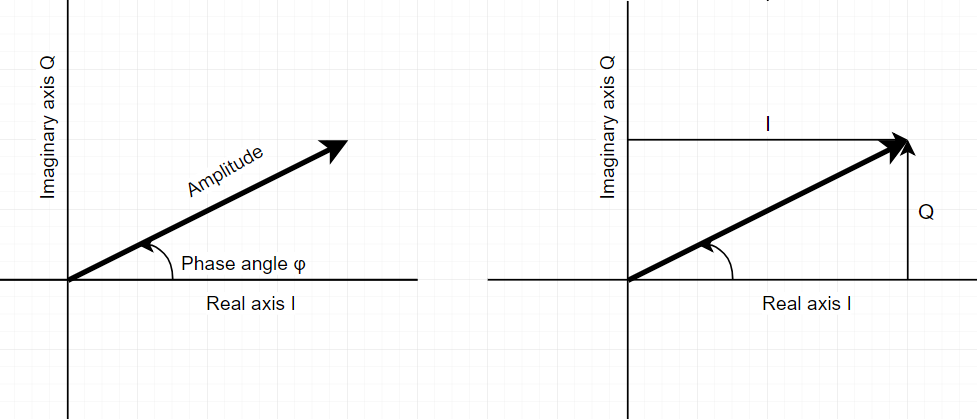
\includegraphics[width=\textwidth]{plots/polarplots.png}
    		\caption{\textit{Representation of sine wave in complex plain}}
    		\label{fig:polarplot}
		\end{figure}
		
		\newpage
		Using trigonometry, the polar coordinates can be converted into I and Q components of the signal using
		equations:
		\begin{itemize}
			\item $I = A cos\left(2\pi f t\right)$, \label{eq:IQ}
			\item $Q = A sin\left(2\pi f t\right)$,
		\end{itemize}
		
		IQ data model is widely used in RF communication systems. It allows to distinguish type of modulation used 
		on carrier. Allows to introduce concept of positive and negative frequency. Amplitude and phase angle form
		seems to be more intuitive, however precisely varying the phase of a high-frequency carrier sine wave in a
		hardware circuit according to an input message signal is difficult. Therefore such hardware modulators will
		be expensive and hard to design and build. To avoid direct modulation of RF signal phase signal is decomposed
		to I and Q components.
		\\
		
		According to Ptolemy’s identitie for the cosine of sum sine wave carrier can be represented as:
		\[
			Acos\left(2\pi ft + \phi\right) = Acos\left(2\pi ft\right)cos\left(\phi\right) - Asin\left(2\pi\right). ft)sin(\phi)
		\]
		Using equation \ref{eq:IQ} following formula is obtained:
		\[
			Acos\left(2\pi ft + \phi\right) = I cos\left(2\pi f t\right) - Q sin\left(2\pi f t\right),
		\]
		where:
		\begin{itemize}
			\item I - is amplitude of in-phase signal,
			\item Q - is amplitude of quadrature signal.
		\end{itemize}
		
		Using this data samples representation, modulation of phase of the RF signal is possible just by modulation of
		I/Q signals amplitudes and then mix it with carrier and quadrature of carrier using mixers. Schematics below 
		shows structure of IQ modulator and demodulator.
		
		\begin{figure}[!htb]
    		\centering
   			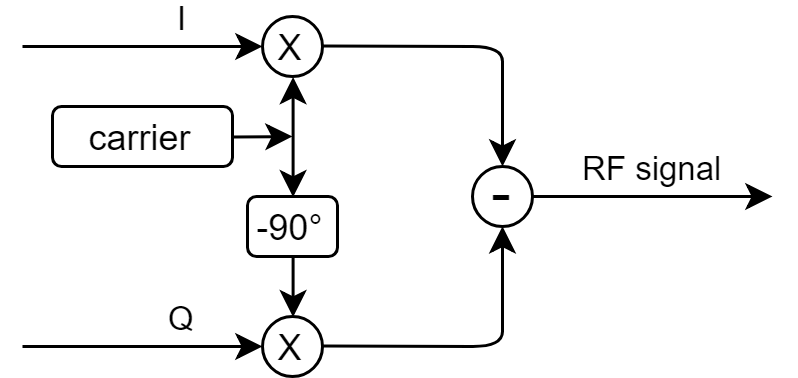
\includegraphics[width=\textwidth]{images/iqmod.png}
    		\caption{\textit{Schematic of IQ modulator}}
    		\label{fig:polarplot}
		\end{figure}
		
		\begin{figure}[!htb]
    		\centering
   			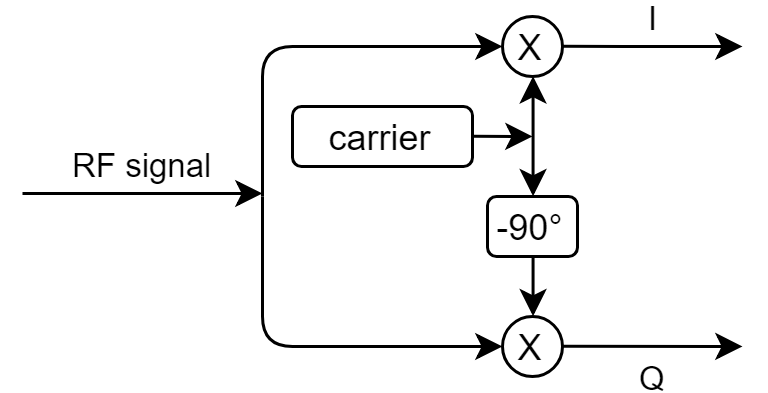
\includegraphics[width=\textwidth]{images/iqdemod.png}
    		\caption{\textit{Schematic of IQ demodulator}}
    		\label{fig:polarplot}
		\end{figure}
		\newpage
		The flexibility and simplicity of this solution compared to direct phase manipulations
		is a reason why I/Q modulators and demodulators are so widely used and popular in RF hardware.
		

	\section{IQ imbalance models}
	\section{Software Defined Radio}
		SDR (Software Defined Radio) is a radio communication system where components typically implemented in hardware (e.g. mixers, filters, amplifiers, modulators/demodulators), are instead implemented by the means of software. 
\chapter{Hardware and tools}
	\section{Zynq and Xilinx tools}
	\section{Adalm Pluto and AD tools}
	\section{Simulation environment}
	
\chapter{Algorithms}
	\section{DC offset correction}
		Moving average filter and Gaussian filter
	\section{Magnitude correction}
	\section{Phase correction}
		Blind phase correction algorithm

\chapter{Simulations}
Chapter with all algorithms simulation in Matlab.
	\section{Single tone signal}
	\section{Multitone signal}
	\section{QAM modulation}
	
\chapter{Measurements}
Chapter with all algorithms implemented in Zynq PL.
	\section{Single tone signal}
	\section{Multitone signal}
	\section{QAM modulation}


\chapter{ Conclusions}


\addcontentsline{toc}{chapter}{Bibliography} %utworzenie w spisie treści pozycji Bibliografia
\bibliography{bibliografia} % wstawia bibliografię korzystając z pliku bibliografia.bib - dotyczy BibTeXa, jeżeli nie korzystamy z BibTeXa należy użyć otoczenia thebibliography

\begin{thebibliography}{9}
\bibitem{highSpeedDesign} 
Stephen H. Hal, Garrett W. Hall, and James A. McCall. 
\textit{High-Speed Digital System Design - A Handbook of Interconnects Theory and Design Practices}.
New York, Chichester, Weinheim, Brisbane, Singapore, Toronto, 2000.


\end{thebibliography}
%opcjonalnie może się tu pojawić spis rysunków i tabel
% \listoffigures
% \listoftables
\end{document}
